\documentclass[journal]{IEEEtran}
\usepackage{cite}
\usepackage{graphicx}
\usepackage{amsmath}
\usepackage{mathtools}
\usepackage{booktabs,ragged2e}
\usepackage[flushleft]{threeparttable}
\renewcommand\TPTtagStyle{\textit}
\usepackage[strings]{underscore}
\usepackage{minted}
\usepackage{subfigure}
\hyphenation{op-tical net-works semi-conduc-tor}
\usepackage[british]{babel}
\usepackage[hidelinks, unicode]{hyperref}

\begin{document}
\BeforeBeginEnvironment{minted}{\medbreak}
\AfterEndEnvironment{minted}{\medbreak}

\title{Feature Detection and Tracking}

\author{Samuele Bortolotti (229326), Department of Information Engineering and Computer Science, University of Trento\\
\href{mailto:samuele.bortolotti@studenti.unitn.it}{\texttt{samuele.bortolotti@studenti.unitn.it}} }

\maketitle

\begin{abstract}
The automated use of unique and quantifiable data to detect the presence, recognize, or define the behavior of objects in a scene has been researched extensively in the computer vision field. When examining a scene, it is appropriate to seek for relevant characteristics, such as colors, forms, and edges, in order to adequately outline the object motion. 

The purpose of this report is to present a feature detection and tracking framework for classical computer vision feature descriptors, as well as to describe implementation choices and to offer a qualitative review of feature detector performance, while presenting my point of view. This study focuses on the implementation of the Lucas-Kanade optical flow and Kalman filter tracking methods, as well as certain feature recognition algorithms ranging from simple blobs and corners to more robust and current algorithms such as SIFT and ORB.
\end{abstract}

\begin{IEEEkeywords}
Feature detection, feature tracking, Kalman filter, Lucas-Kanade optical flow, SIFT, ORB
\end{IEEEkeywords}

\IEEEpeerreviewmaketitle


\section{Introduction}

\IEEEPARstart{T}{he} aim of this report is to implement and test the performances of at least two different feature detectors complemented with a tracking algorithm. 

As for tackling the assignment, the paper ranges from the most basic features, such as corners and shapes, to more elaborated ones such as SIFT and ORB.
To be precise, the report pursues its aim using traditional computer vision handcrafted features rather than pre-trained artificial neural networks' feature extractors. Although the results may have been slightly worse, they are still remarkable, demonstrating why those approaches are still legitimate and extensively used. As a matter of fact, the choice of the descriptor derives from my curiosity in observing how naive and sophisticated detected feature points differ. Instead, as for tackling the tracking of the features, the Lucas-Kanade optical flow and the Kalman filter were employed.

In order to evaluate the performances of the feature detectors and trackers, it has been provided a benchmark video.

~\hyperref[tab:video]{Table I} shows some of the video basic statistics.

\begin{table}[h]
\centering
\caption{Benchmark video base statistics}
\label{tab:video}
\setlength\tabcolsep{0pt}
\begin{tabular*}{0.6\columnwidth}{@{\extracolsep{\fill}}ll}
\toprule
    Property & Value \\ 
\midrule
    Bit rate & 25.1 Mb/s \\
    Width & 2 160 pixels \\
    Height & 3 840 pixels \\
    Sampling rate & 48.0 kHz \\
    Frame rate & 46.875 FPS \\
    Duration & 30s 597 ms \\
\bottomrule
\end{tabular*}
\end{table}

Such video contains several challenges which must be considered while constructing both the detection and tracking phases. The scenario depicts an industrial context with glossy surfaces, perhaps more than one light source, shadows, repeated patterns, red led flashing and a non linear camera movement. 

\begin{figure}
    \centering
    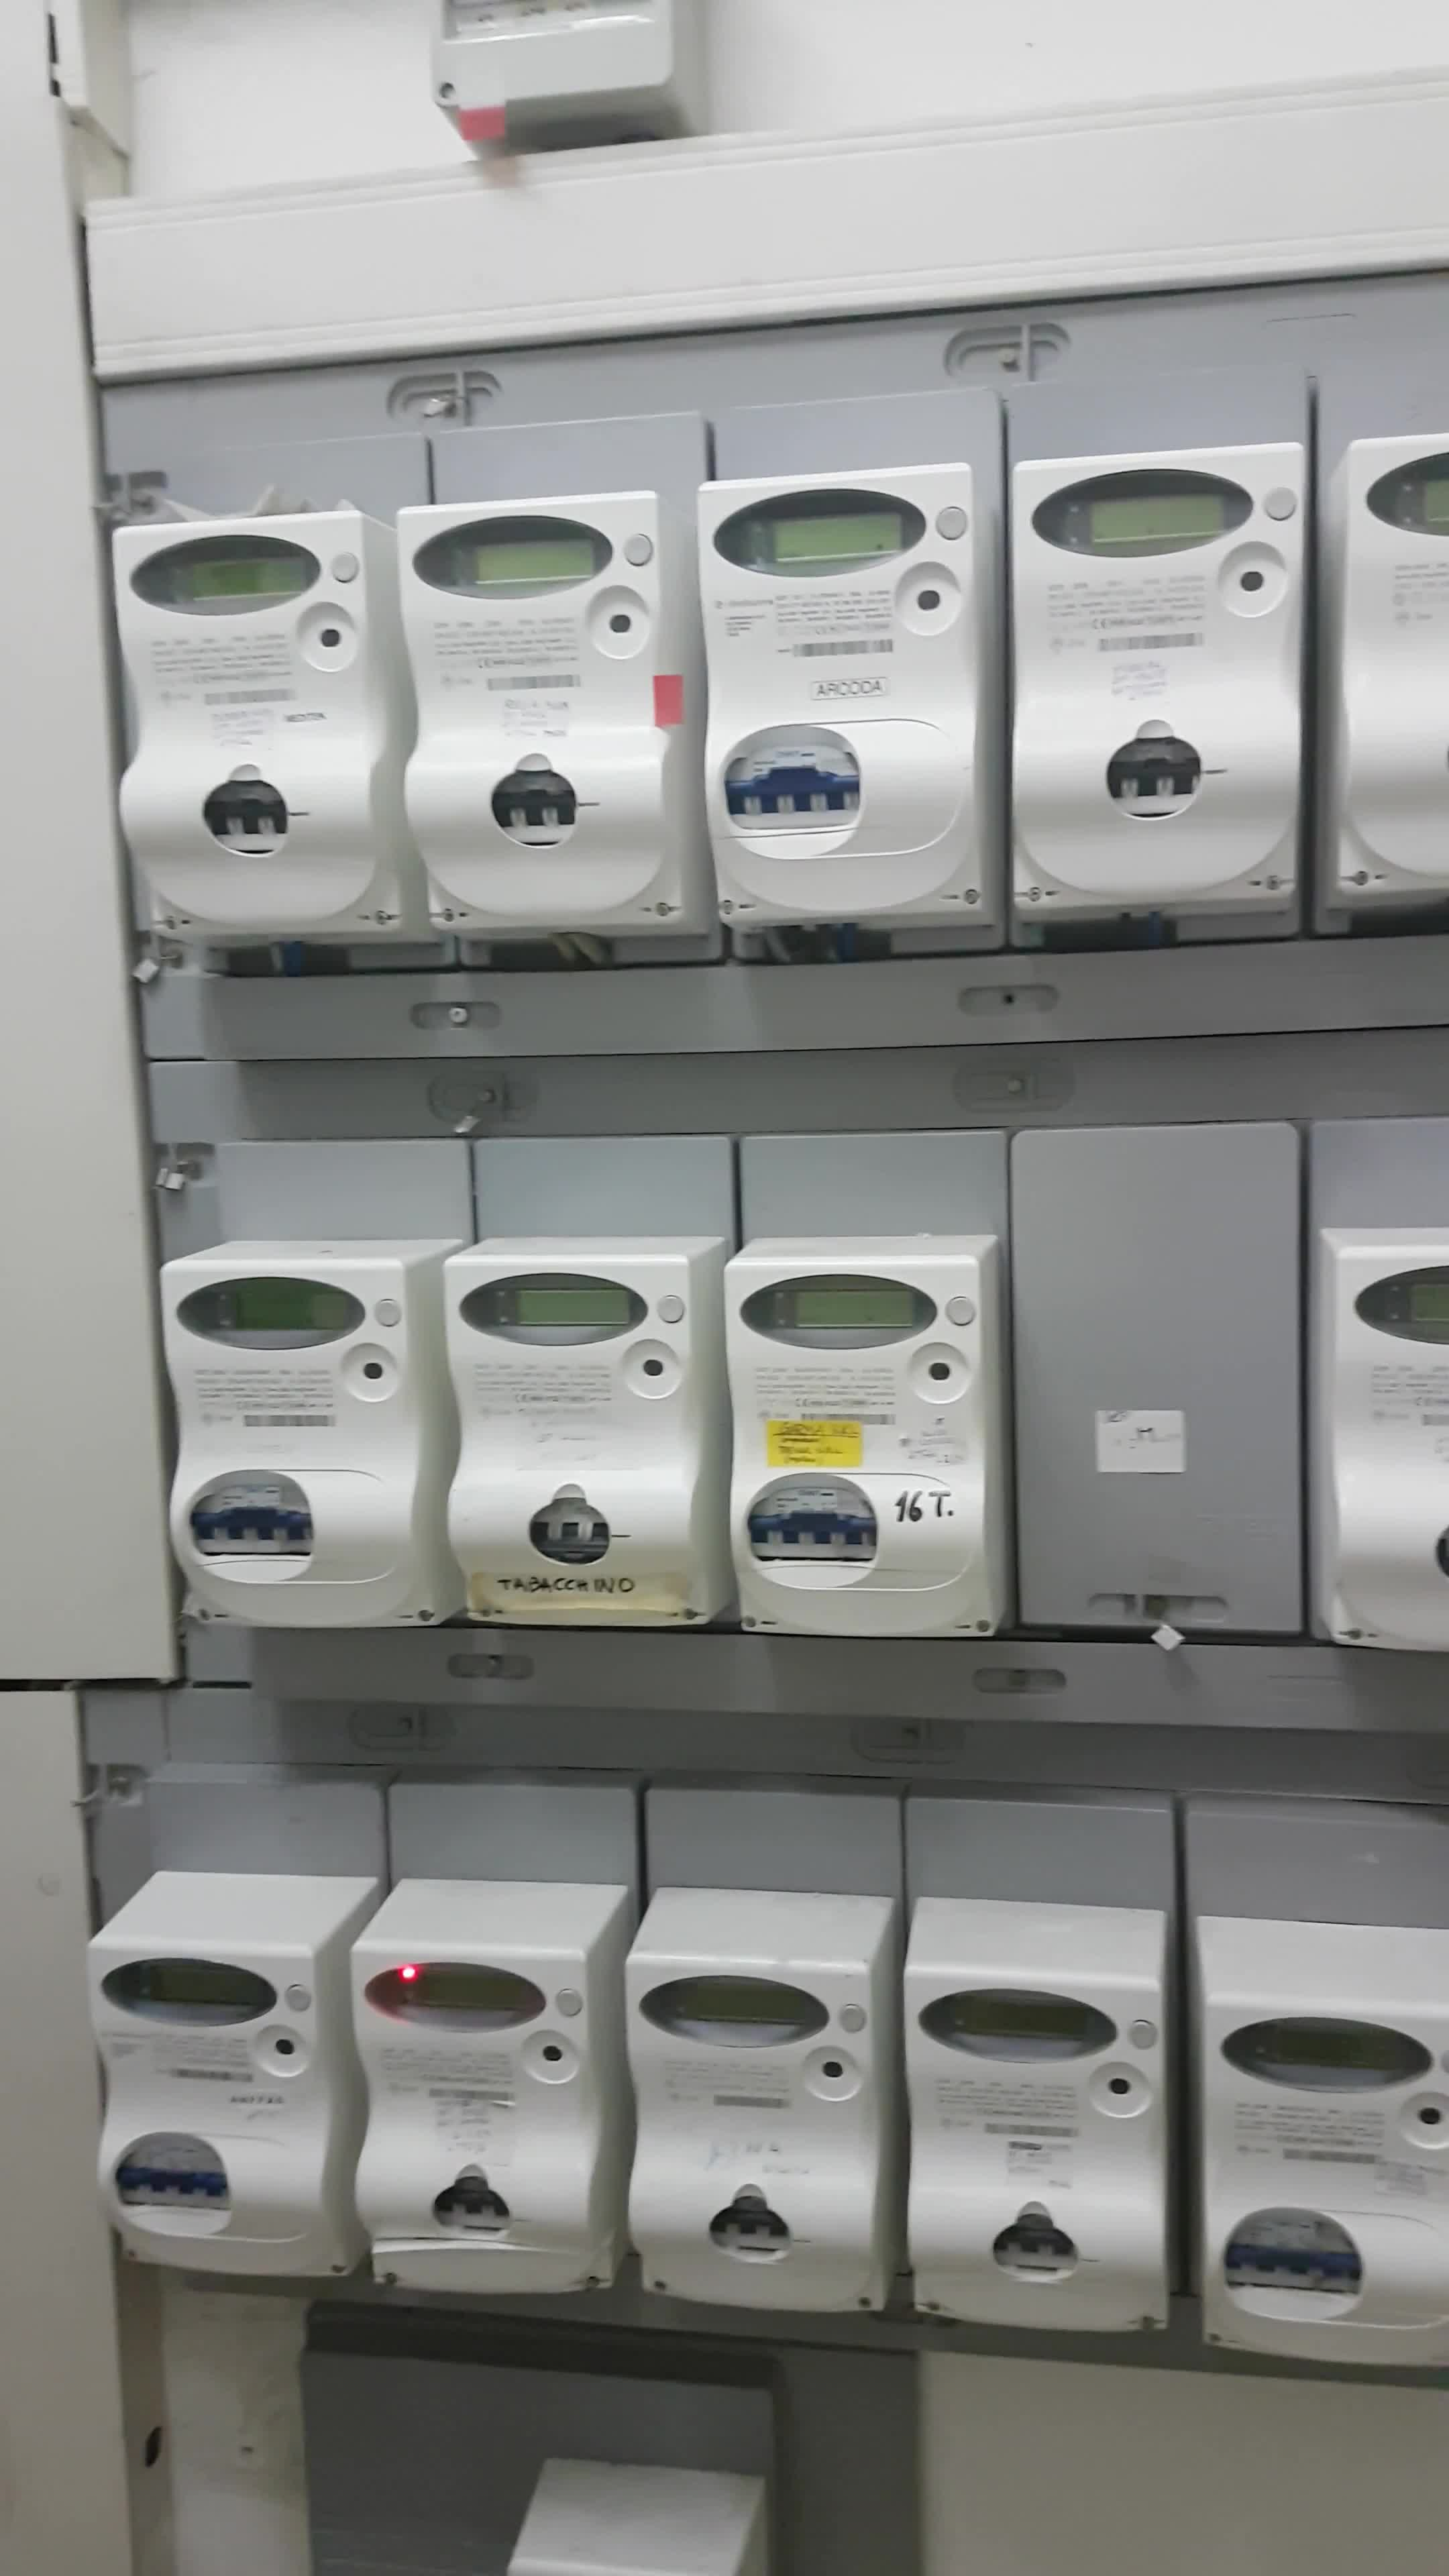
\includegraphics[height=2in]{images/contesto_industriale.jpg}
    \caption{Frame of the benchmark video ContestoIndustriale1.mp4}
    \label{fig:contestoindustriale}
\end{figure}

From a very rough point of view, it is expected the basic feature detectors to perform poorly. 
Most likely due to the items in the scene which are identical to one another; indeed blobs solely on forms and colors are expected to perform a sub-optimal feature detection. Furthermore, due to lighting difficulties, corner-based descriptors may identify spurious contours. As elementary as it may seem, it is expected that more robust feature descriptors such as SIFT and ORB yield the best qualitative results, considerably better than the simpler feature detection methods.

Moreover, since the camera motion is not linear, it is expected the Kalman filter to have difficulty while forecasting the appropriate movement of the features because it is based on the assumption that the process and the measurement models are linear. As the reader may have guessed by now, the feature detectors and trackers' settings are critical for the fulfillment of the assignment in a such difficult environment. 

This paper presents a possible solution of the assignment, as well as the parameters tweaking to overcome most of the issues. In particular, ~\hyperref[sec:featuredetection]{Section II} discusses the employed feature detector methods,~\hyperref[sec:featuretracking]{Section III} provides an overview of the tracking methods and~\hyperref[sec:projectstructure]{Section IV} defines the proposed method and the project architecture details. Finally,~\hyperref[sec:conclusion]{Section V} presents the concluding remarks.

\section{Feature detection}
\label{sec:featuredetection}
For a variety of reasons it is relevant to consider any number of arbitrary, uniquely identifiable and heterogeneous elements inside an image.

Intensively detecting features across different frames is extremely expensive, and constructing an accurate and efficient feature detector which scales in high-resolution video is for sure not trivial.

In this scenario, we are interested in finding relevant aspects of the objects across a temporal interval, which is usually tackled by not computing the features at each frame but leveraging on the scene temporal changes across subsequently frames; by doing so, we usually end up accomplishing feature detection by undertaking motion detection.

In this section it is provided a high level background of the employed feature detectors.

\subsection{Harris corner detector}
Corners, also known as interest points, are relevant since they depict the intersection of two or more edges, which highlights where their direction change. Furthermore, corners are rotation-invariant, namely robust to object rotation; however they are not robust to scale, since if the picture is resized, the corner detector may fail in the identification process~\cite{opencv_library}. 

This report has considered Harris edge detector~\cite{harris1988combined} as an effective way to detect interest points and subsequently feed them to the tracking algorithm. The main idea behind the approach is that corners can be identified by looking seen as a variation in the gradient in the image. As a brief explanation, the Harris corner detector requires a grayscale representation of the picture, then it sweeps a window across the image employing the Sobel operation to determine its intensity variation. Windows with high intensity variations are likely to contain corners; to detect them, the algorithm computes a score for each window, equal to the difference between the window determinant and the square of its trace multiplied with a scaling factor; after that, the score is used to determine the presence of corners according to one threshold.

\subsection{Blob detector} 
A Blob is a group of connected pixels in an image which share some common properties such as color or shape. As it may be intuitive, blobs are strictly parameter dependent, which means that in most of the cases, blobs based on the shape are neither rotation nor scale independent whereas those based on colors suffer from illumination issues.

The OpenCV library~\cite{opencv_library} provides an algorithm to extract blobs from an image which comprises the following steps. First, it converts the source image to a binary image by applying thresholding with several thresholds. Then, it extracts connected components from every binary image and calculates their centers. After that, it groups centers from several binary images by their coordinates, merging close blobs by considering color and proximity. Finally, from the merged shapes, it estimates the centers of blobs and their radiuses and it returns the locations and the sizes of keypoints.

\subsection{SIFT}
Scale Invariant Feature Transform (SIFT)~\cite{lowe2004distinctive} is a robust, scale and rotation invariant feature detection algorithm which aims to extract keypoints and compute its descriptors. 

The algorithm creates a subspace representation of the picture gradually applying a Gaussian smoothing filter, resulting in each image being a blurred version of the preceding one.
An octave is a collection of gradually blurred photographs. The Difference of Gaussian is applied to different octaves of the picture while examining the image at various scales.
Following this, candidate keypoints are discovered by looking for maxima and minima throughout size and space. To achieve picture rotation invariance, each keypoint is assigned to an orientation~\cite{opencv_library}. 

In addition, the keypoints' descriptors are constructed by splitting a 16 by 16 pixel neighborhood surrounding the keypoint into 4 by 4 pixel sub-blocks. An 8 bin orientation histogram is built for each of these sub-blocks. To build a keypoint descriptor, the whole 128 bin values are extracted and represented as a vector.

\subsection{ORB}
ORB~\cite{rublee2011orb} is a rotation and scale invariant alternative to the SIFT feature descriptor, which was built on top of the FAST keypoint detector and BRIEF descriptor.
The algorithm first finds keypoints using the FAST keypoint detector, and then uses the Harris corner detection score to determine the best points among them.

ORB employs a pyramidal implementation to deal with multi-scale features, building the picture representation at different resolutions~\cite{opencv_library}.

ORB uses a modified version of BRIEF to create the keypoint descriptors. The main idea behind the BRIEF feature descriptor is to convert all keypoints into a binary feature vector, which may then be used to classify or recognize the object. The resulting feature vector is a 256 bit string, which describes each keypoint.

\section{Feature tracking}
\label{sec:featuretracking}
During a sequence of photographs illustrating the temporal development of a scene, feature tracking refers to keep track of one or more feature points, generally by presuming that the change is gradual enough for the item to be near where it was in the previous frame.

Due to noise, shadows, splitting, merging, occlusions, or other difficulties, the algorithm ability to generate a consistent representation may deteriorate overtime.

In this section I provide an high level background of the employed motion trackers.

\subsection{Lucas-Kanade Optical Flow}

The Lucas-Kanade optical flow algorithm~\cite{lucas1981iterative} is a efficient method to get optical flow information. It works under the assumption that the pixels aspect does not considerably change across two consecutive frames and that the objects' displacement vectors are minimal in that interval. By examining variations in pixel intensity within a particular window, the Lucas-Kanade algorithm finds the best match withing a neighborhood.

Usually, when we are talking about the Lucas-Kanade algorithm we refer to its pyramidal implementation, which builds a pyramid of images progressively downsampled. To perform the tracking, the algorithm first considers the matches in the lower detailed picture and then it continuously refines the displacement vector with finer details images.

\subsection{Kalman Filter}
The Kalman filter~\cite{kalman1960new} is a tracking algorithm which leverages on a sequence of measurements taken over time to provide estimations of the next object's location, assuming that both the measurement and the process noise follow a Gaussian distribution.

The Kalman filter generates estimates of the current state variables, as well as their uncertainty, for the prediction phase. Once a new observation is given, the estimates are updated using a weighted average.

\section{Proposed method}
\label{sec:projectstructure}
In order to organize the code in a modular way, the repository is organized in sub-modules within a unique module \emph{fdt} (shorthand for feature-description-and-tracking). 

Such organization has allow to test each of the main functionality employed in the final result individually, which not only gives a comprehensive overview of each technique, but also allows to better fine-tune the methods parameters.

To facilitate the comprehension, Figure~\ref{fig:repository} portraits the main functionality which the code can carry out. 

\begin{figure}
    \centering
    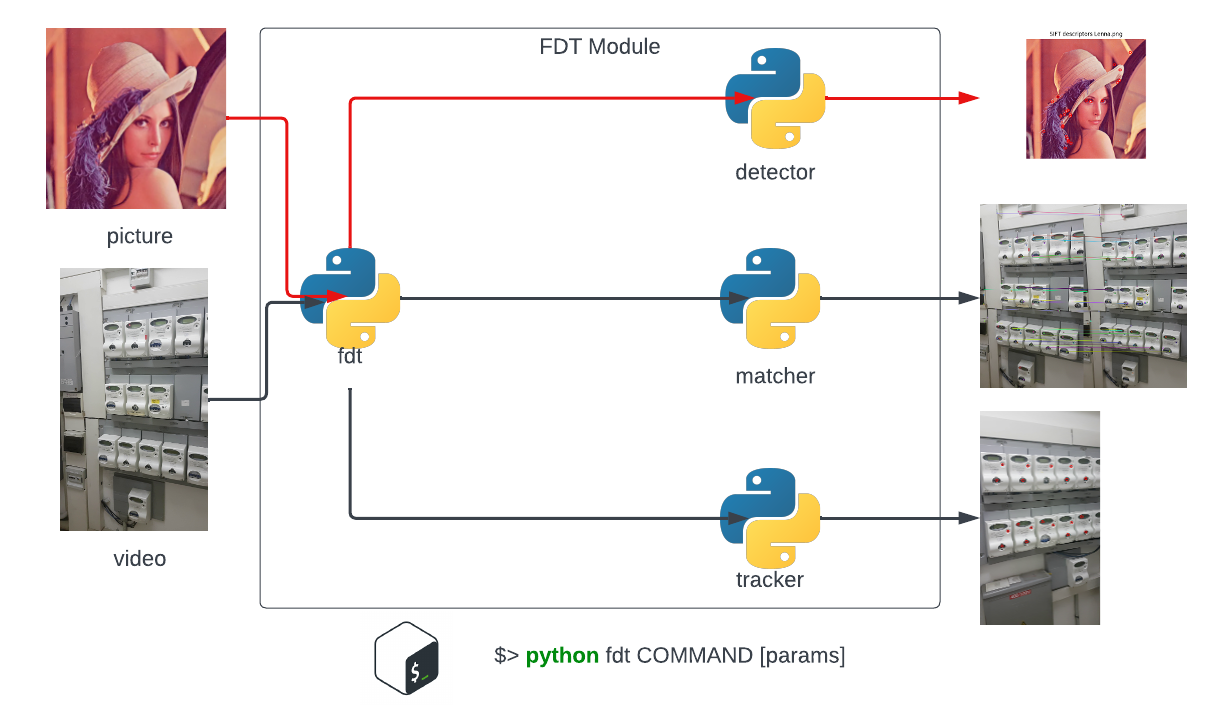
\includegraphics[angle=270,origin=c,width=2.5in]{images/structure.png}
    \caption{Repository structure}
    \label{fig:repository}
\end{figure}

In this section, these functionalities will be discussed as well as the parameter selected.

\subsection{Detectors}
The implemented detectors are HarrisDetector, SimpleBlobDetector, SIFT and ORB, which are all provided by the OpenCV library.

All the detectors model are present under the \emph{detection} folder and take the path of an image as a parameter. Moreover, as a feature of the Python SubParser class, the proper parameter can be passed as command line arguments:

\begin{minted}{bash}
$> python -m fdt $FUNCTION $PARAMETERS
\end{minted}

To see different aspects of the feature detectors, two test images are provided, one is the standard test image used in the field of image processing, Lena Forsèn, the other one portraits an industrial lime kiln surrounded by trees. The selection of these two images lies on the fact that the image of Lena has several smoothed surfaces and few textures in the hat. The photograph of the lime kiln is characterized by continuous textures and angles; in a such complex environment, it is difficult to find only few significant features.

Furthermore, for both the Harris corner detector and the Blob corner detector it is possible to modify a configuration file, which can be found under the \emph{config} folder. In order to use it, the function needs to be called with \emph{$--$config-file} flag set.

\subsubsection{Harris corner detector}

The OpenCV Harris corner detector relies on 4 parameters, namely block\_size, k\_size, k and threshold, which are respectively the size of the neighborhood considered for corner detection, the aperture parameter of the Sobel derivative, the Harris detector free parameter in the equation and the multiplicative constant for the threshold.

Following considerable manual tweaking, the result of the setting for both photos and video is shown in Figure~\ref{fig:harris}.

\begin{itemize}
    \item $block\_size$: the increment of this value implies bigger receptive fields for corner detection, which means larger and consequently less precise detected keypoints. This value is set to a relative small quantity.
    \item $k\_size$: emphasizes more significant corners when it lies in between values from 9 to 15.
    \item $k$: according to the documentation it should be a value in between 0.04 and 0.06. This value has been set to 0.04.
    \item $threshold$: due to the fact that it is totally dependent on what we want the algorithm to detect, the threshold is arguably the most hardest parameter to define. A suitable value under the situations which has been considered is 0.1.
\end{itemize}

\begin{figure}
\centering
    \subfigure[]{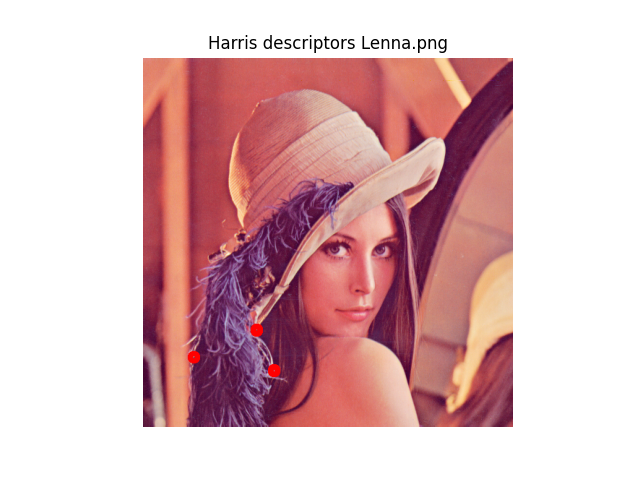
\includegraphics[width=0.23\textwidth]{images/harris_lenna.png}}
    \subfigure[]{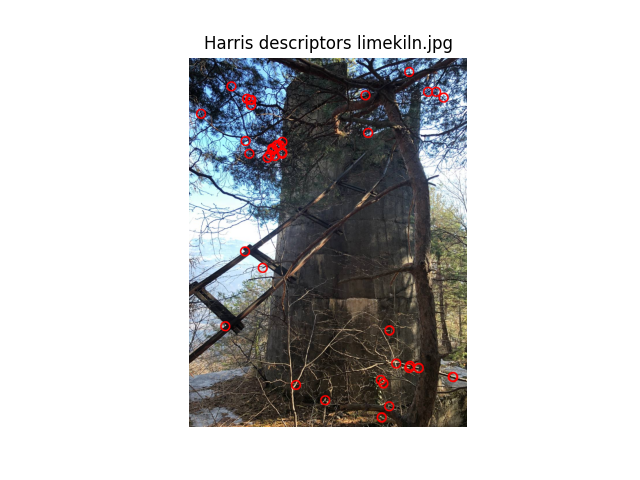
\includegraphics[width=0.25\textwidth]{images/harris_lk.png}}
    \caption{(a) Harris features on Lena Forsén image (b) Harris features on the lime kiln}
    \label{fig:harris}
\end{figure}

To summarize, the final configuration is the one depicted below:

\begin{minted}{python}
# Harris corner detector
current_conf = {
    "block_size": 2,
    "k_size": 9,
    "k": 0.04,
    "thresh": 0.2,
}
\end{minted}

Concerning the test video, employing both the Kalman filter and the Lucas-Kanade optical flow, the arrangement has produced acceptable visual results.

As a major disadvantage, the highlighted points are typically grouped together in the same place, making most of the critical points redundant.

\subsubsection{Blob detector}
As far as the blob detector concerns, the OpenCV Simple Blob Detector allows to declare a set of criteria to accomplish blob selection.

Such criteria are: 
\begin{itemize}
    \item color: the intensity of a binary image in the center of a blob is compared to the specified color.
    \item area: the blobs are sought within a given shape defined by the flags \emph{minArea} and \emph{maxArea}.
    \item circularity: the blob should exhibit a circularity comprised between a minimum and a maximum.
    \item convexity: the area of the blob convex hull should be between a minimum and maximum convexity.
    \item ratio: the blobs ratio of inertia. 
\end{itemize}

According to how the video scenario is concerned, color does not seem to be a relevant feature to track, since as it can be seen in Figure~\ref{fig:contestoindustriale} the objects have basically the same colors of the background. Moreover, due to the presence of shadows, it may be possible to detect blobs around objects which do not exist. Therefore, the blob extraction phase has been based on the shapes of the objects around the scenes.

As a result, the most remarkable characteristics, in my opinion, are the circular-shaped buttons, levers and nails on the industrial objects.
Starting with this fundamental assumption, I enabled filtering by area of the discovered blob by setting a high amount of minimum circularity so as to filter out the shapes which are not interesting.
Furthermore, the important spots are all convex, as I stated at the beginning of the section, thus I have instructed the detector to always reject concave forms.
Finally, since the forms aren't particularly elongated, the inertia ratio is set relatively high to favor designs which are more compact.

\begin{figure}
\centering
    \subfigure[]{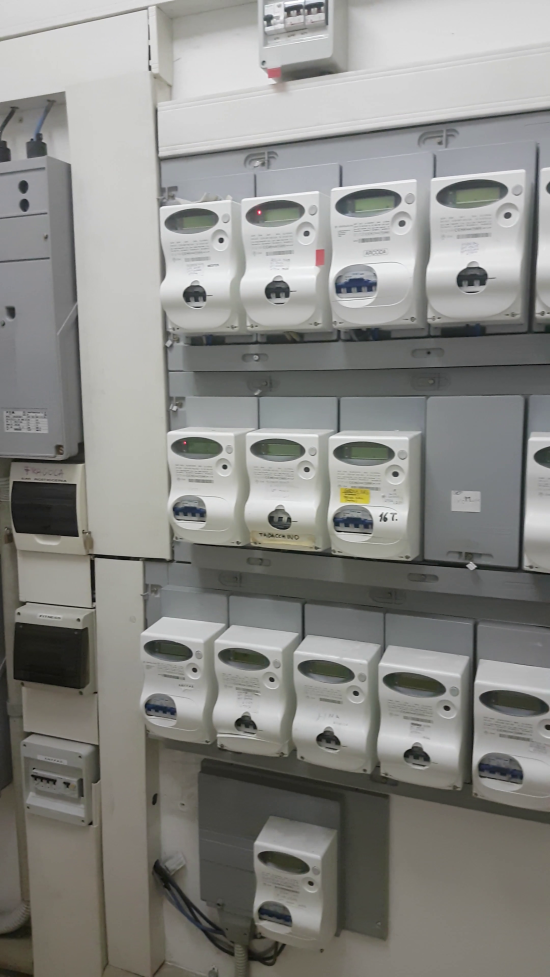
\includegraphics[width=0.15\textwidth]{images/scene.png}}
    \subfigure[]{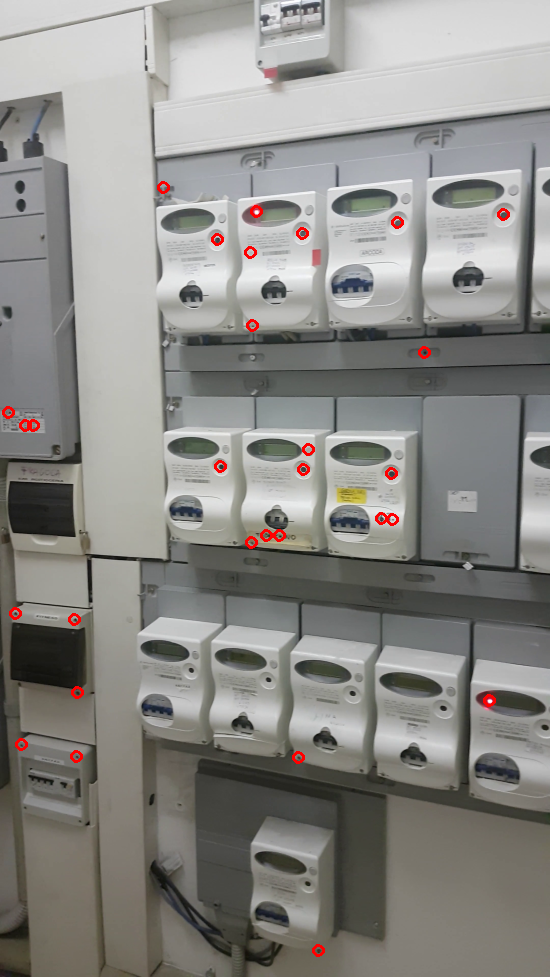
\includegraphics[width=0.15\textwidth]{images/blob_scene.png}}
    \caption{(a) Contesto_Industriale test frame (b) Blob keypoints on the test frame}
    \label{fig:blob}
\end{figure}

The result of the tweaking is shown in Figure~\ref{fig:blob}. Thus, to summarize the final configuration of the blob detection algorithm is the following:

\begin{minted}{python}
# Current Simple Blob extractor
current_conf = {
    "filterByColor": False,
    "blobColor": 0,
    "filterByArea": True,
    "minArea": 3.0,
    "maxArea": 500.0,
    "filterByCircularity": True,
    "minCircularity": 0.8,
    "maxCircularity": int_inf,
    "filterByConvexity": True,
    "minConvexity": 1.0,
    "maxConvexity": int_inf,
    "filterByInertia": True,
    "minInertiaRatio": 0.7,
    "maxInertiaRatio": int_inf,
    "minThreshold": 0,
    "maxThreshold": 255.0,
    "thresholdStep": 5,
    "minDistBetweenBlobs": 8.0,
    "minRepeatability": 2,
}
\end{minted}

As may be elementary by the previous analysis, the concept of a salient point and its associated configuration is entirely handcrafted to detect those precise shapes and it is undoubtedly sub-optimal in situations different from the one tested. As a matter of fact, the current configuration will detect more shapes in the other test images. Despite this, the features were evenly distributed across the various frames of the video, not clustering in specific spots, and the detector was able to track small nails or the buttons of the industrial object for the majority of the time, which may be the most basic element to track the element position. Nonetheless, still noisy dots around the objects labels were detected probably due to the text contained therein, which makes this approach the less performing one from a qualitative viewpoint. Furthermore, when the camera points at the boxes from a different perspective, the blob detector struggles to find the relevant point, which is a consequence of the fact that blobs are not resilient to rotation.

\subsubsection{SIFT}

The OpenCV SIFT feature detector is based on the number of features, the number of octaves, the edge threshold, and the sigma value. 

This feature detector has been adjusted based on both the test photos and the given video, such as the previous feature detectors. According to my experience, the ideal number of features to use with the SIFT feature detector method is 35. However, for the Kalman filter 200 features are employed.

The sigma value is set to be 1.6, which is the one of the default configuration, because I've seen that raising sigma degrades the detector's performance in terms of processing time, and no qualitative gains have been discovered to justify such a long computational time.
Instead, raising the number of octaves has resulted in a significant improvement in the final visual result (Figure~\ref{fig:sift}), which has now been increased from 5 to 8. 

\begin{figure}
\centering
    \subfigure[]{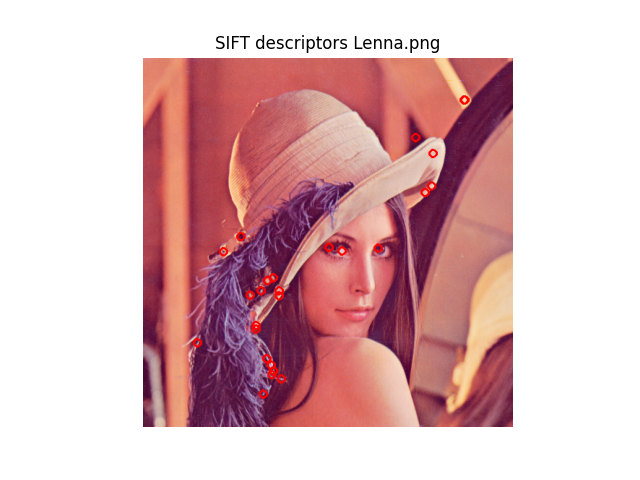
\includegraphics[width=0.23\textwidth]{images/sift_lenna.png}}
    \subfigure[]{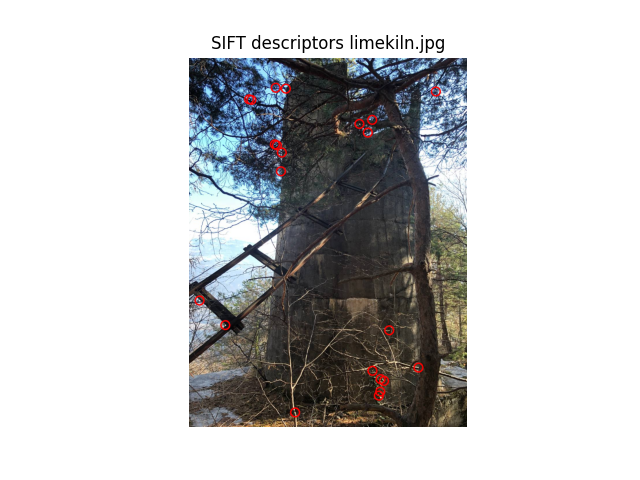
\includegraphics[width=0.25\textwidth]{images/sift_lk.png}}
    \caption{(a) SIFT features on Lena Forsén image (b) SIFT features on the lime kiln}
    \label{fig:sift}
\end{figure}

\begin{minted}{python}
# Current SIFT feature extractor
current_conf = {
    "nfeatures": 35,
    "nOctaveLayers": 8,
    "contrastThreshold": 0.04,
    "edgeThreshold": 10,
    "sigma": 1.6
}
\end{minted}

From what I was able to observe, the feature points retrieved by SIFT are more accurate than any other descriptors I have tried. However, it is computationally heavy, therefore it is extremely difficult to extract the features from each frame; thus SIFT is not effective for low powered devices. However, for applications which require precise features and comply with such computational capabilities, it may obtain remarkable results.

\subsubsection{ORB}

Following the idea of the previous sections to tune the feature detectors, 100 features is a reasonable number to perform the tracking in the test video. Moreover, since no significant improvement was observed, the default values were used. However, for the Kalman filter 200 features are employed.

\begin{minted}{python}
# Current ORB feature extractor
current_conf = {
    "nfeatures": 100,
    "scaleFactor": 1.2,
    "nlevels": 8,
    "edgeThreshold": 31,
    "firstLevel": 0,
    "WTA_K": 2,
    "scoreType": ORB::HARRIS_SCORE,
    "patchSize": 31,
    "fastThreshold": 20 

}
\end{minted}

A visual result is shown in Figure~\ref{fig:orb}.

\begin{figure}
\centering
    \subfigure[]{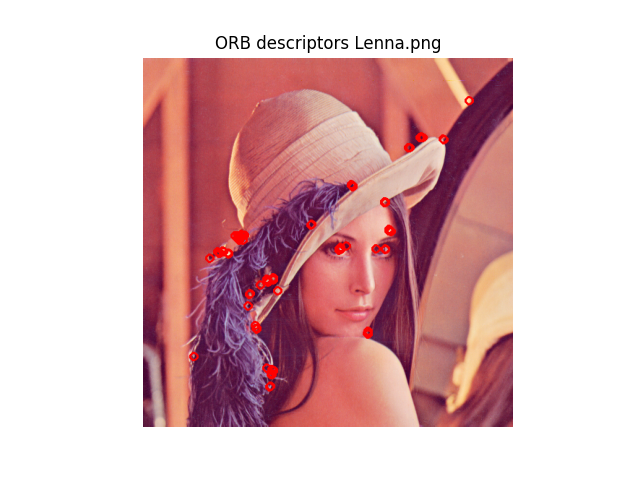
\includegraphics[width=0.23\textwidth]{images/orb_lenna.png}}
    \subfigure[]{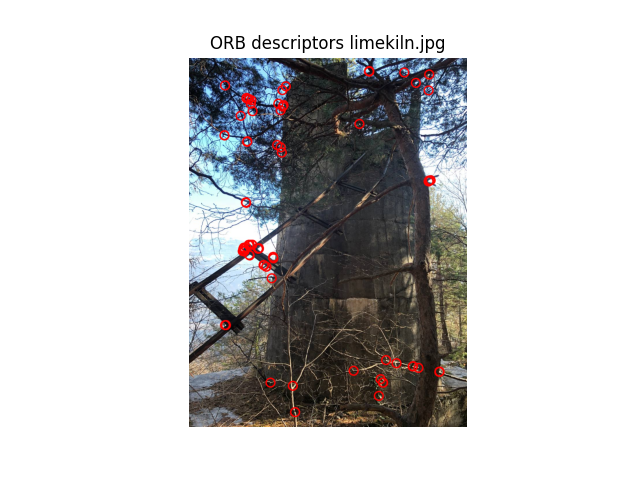
\includegraphics[width=0.25\textwidth]{images/orb_lk.png}}
    \caption{(a) ORB features on Lena Forsén image (b) ORB features on the lime kiln}
    \label{fig:orb}
\end{figure}

The first noticeable distinction from other feature detectors is the detection speed; it is not difficult to run the ORB feature detection repeatedly across subsequent frames.
Furthermore, it produces keypoints which are far more consistent than those obtained by the Harris corner detector and the basic blob detector.

In terms of quality, the more important keypoints are all recognized, albeit there may be points which are detected numerous times, resulting in areas of congested keypoints. As a result, significantly more keypoints are necessary for ORB to identify almost the same areas of interest detected by SIFT. 

Finally, since ORB is significantly quicker than SIFT, it may be a viable choice in low-power devices, as it provides a better trade-off between performance and detection quality. 

\subsection{Trackers}

The Lucas-Kande optical flow and the Kalman Filter are the motion trackers chosen for the assignment.

The feature tracking approach is used by all motion trackers in the tracking folder.

\subsubsection{Lucas-Kanade optical flow}

The calcOpticalFlowPyrLK() function from OpenCV is used in this report so as to implement the Lucas-Kanade optical flow.
I modulated each feature detector to return a pair of elements, specifically the keypoints and their descriptors, in order to adjust the optical flow to any feature detector provided. 

In the default configuration settings, new keypoints are sampled every 50 frames, for the others, the position of the points is inferred from the motion tracking.

As an aside, the motion tracking using Lucas-Kanade optical flow is fairly smooth, and that it is an astonishing way to monitor features in this slowly moving environment under the optical flow assumptions. 

As far as the tracking is concerned, the Lucas-Kanade optical flow is very smooth with the Harris corner detector, the blob detector, and ORB; however with SIFT, the tracking is substantially slower owing to its processing demands. 

A visual comparison of the different features detector using Lucas-Kanade optical flow is shown in Figure~\ref{fig:lucas}.

\begin{figure}
    \centering
    \begin{tabular}{cc}
    \subfigure[]{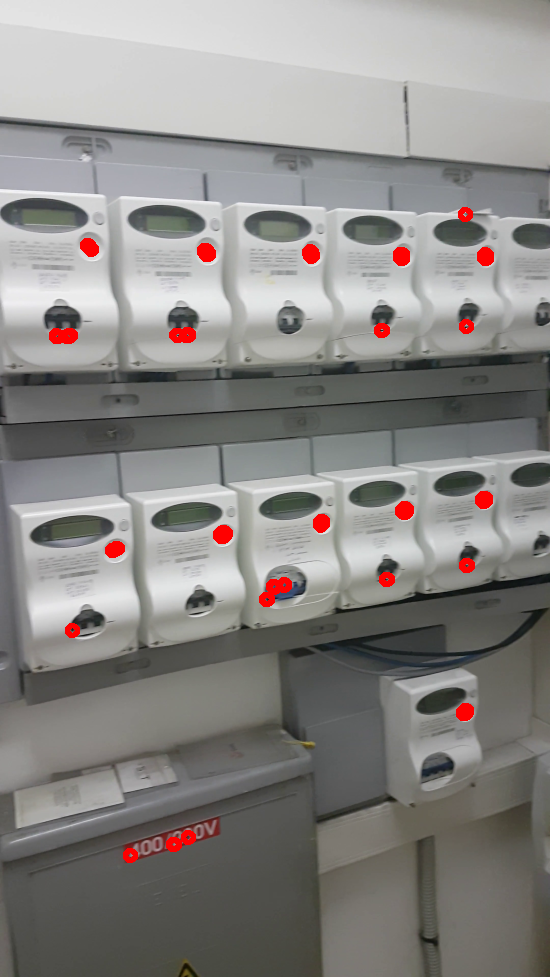
\includegraphics[width=0.15\textwidth]{images/Lucas-KanadeOpticalFlowHarris.png}} &
    \subfigure[]{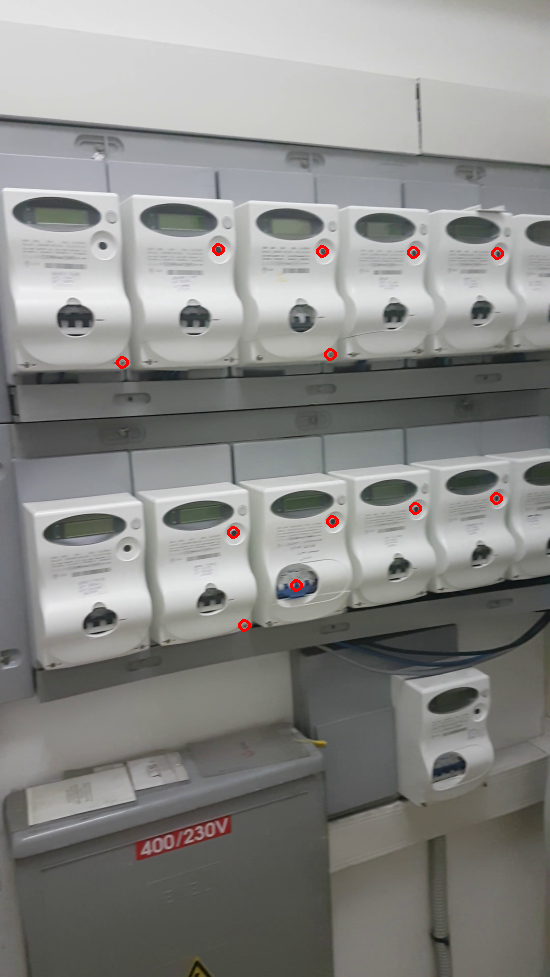
\includegraphics[width=0.15\textwidth]{images/Lucas-KanadeOpticalFlowBlob.png}} \\
    \subfigure[]{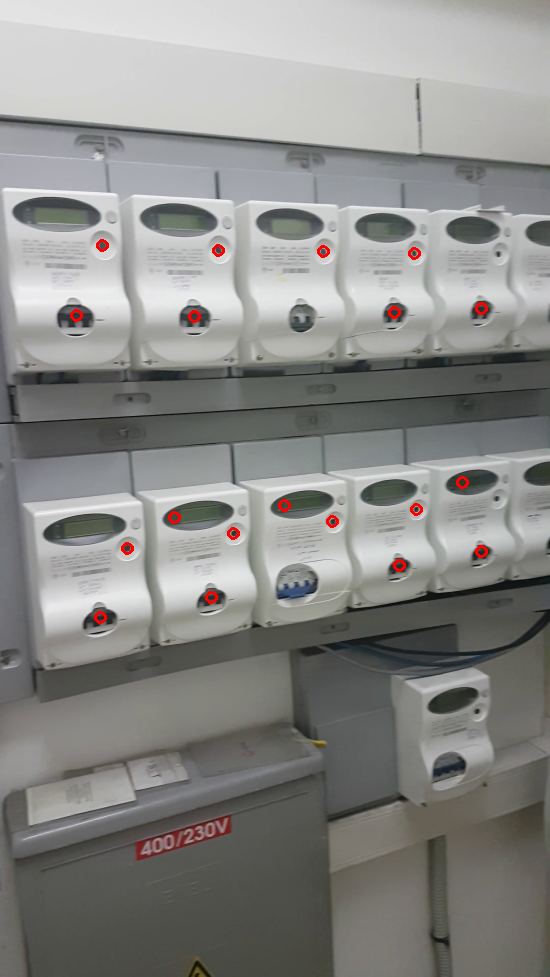
\includegraphics[width=0.15\textwidth]{images/Lucas-KanadeOpticalFlowSIFT.png}} &
    \subfigure[]{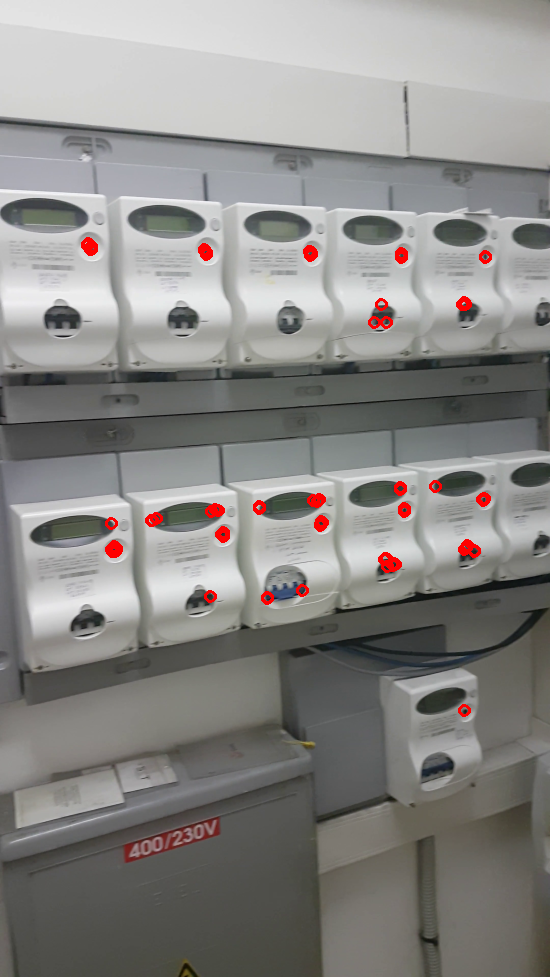
\includegraphics[width=0.15\textwidth]{images/Lucas-KanadeOpticalFlowORB.png}} \\
    \end{tabular}
    \caption{(a) Lucas-Kanade tracking with Harris corner detector (b) Lucas-Kanade tracking with Blob detector (c) Lucas-Kanade tracking with SIFT detector (d) Lucas-Kanade tracking with ORB detector}
    \label{fig:lucas}
\end{figure}

\subsubsection{Kalman}

To update the error covariance matrices and update the prediction, the Kalman filter requires observations.
However, due to the lack of other sensors such as infrared or GPS to determine the precise location of the item, this has been an arduous problem to overcome.

To deal with missing observations, the paper employs a Brute Force Matcher, which determines the correspondences between current and reference descriptors by attempting to mach all of the target descriptors. In order to simulate observations and thus descriptors, the method runs the feature extractor at each frame, which is a computationally intensive process. 

The matcher is then applied to each current descriptor in order to accurately map the target descriptors to the reference descriptors and utilize this new configuration as a ground-truth to update the Kalman filter matrices.
However, this has caused several issues with two of the descriptors I chose to address the assignment; in particular, neither the Harris corner detector nor the blob detector are associated with descriptors, hence I had to rely on the SIFT descriptors computed on the keypoints retrieved by the previously defined method to implement this method. 

The main challenge of the whole pipeline has been to tune correctly the Kalman filter matrices. As stated in the report introduction, this tracking algorithm works under the assumption of linear movement which is not exactly the scenario depicted in the paper. During the development of the assignment I have seen that increasing the process and measurement noise to a high values causes the forecast to assess quickly.
Furthermore, the Kalman filter has demonstrated to be resilient after the initial assessment step, even if the matcher is not always exact in monitoring the relevant characteristics. However, some flickering can still be observed probably due to the matcher failure deriving from flat or repetitive patterns in a challenging environment.

Finally, due to the descriptors that are required at every frame, the entire pipeline I have built up is exceedingly sluggish, making it unsuitable for SIFT. Furthermore, the Kalman filter does not converge quickly when there are few and sparse data, as seen by the small number of features detected by the blob extractor. When the number of characteristics, and hence observations rises, the findings become considerably more consistent. For this reasons Kalman filter with the blob detectors works really poorly.

A visual comparison of the different features detector using the Kalman filter is shown in Figure~\ref{fig:kalman}.

\begin{figure}
    \centering
    \begin{tabular}{cc}
    \subfigure[]{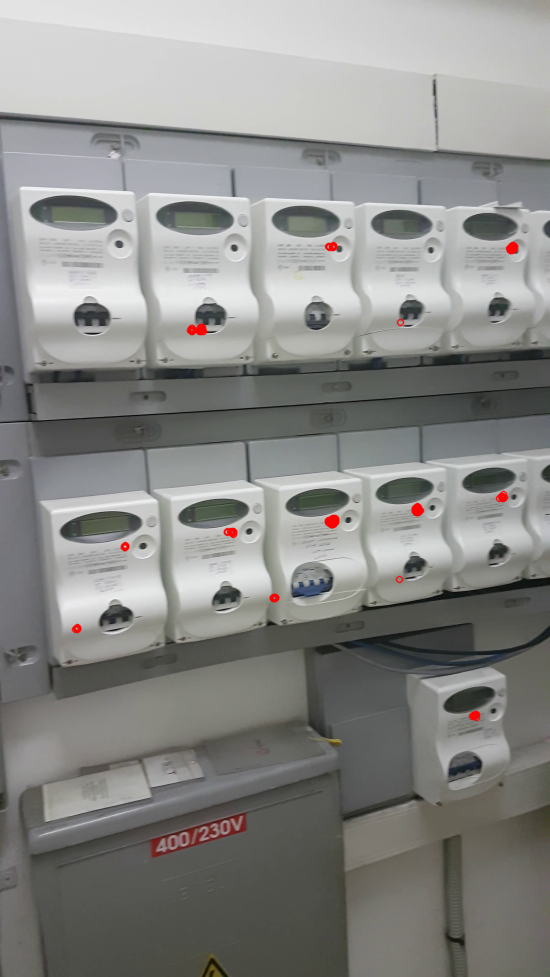
\includegraphics[width=0.15\textwidth]{images/KalmanHarris.png}} &
    \subfigure[]{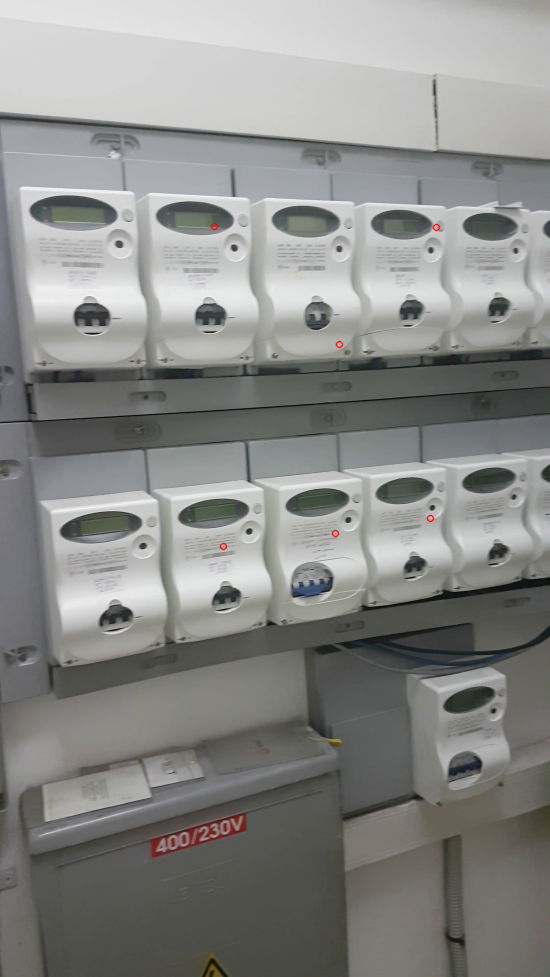
\includegraphics[width=0.15\textwidth]{images/KalmanBlob.png}} \\
    \subfigure[]{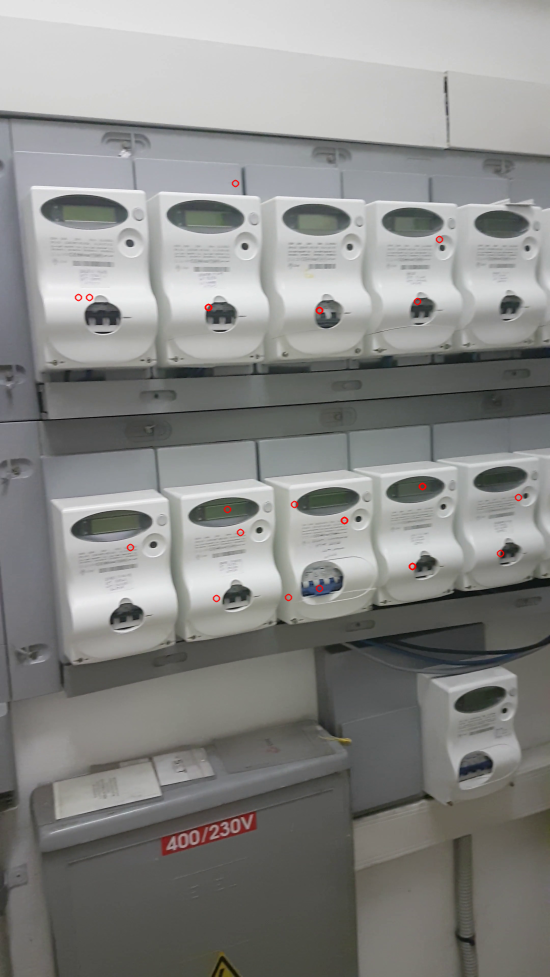
\includegraphics[width=0.15\textwidth]{images/KalmanSift.png}} &
    \subfigure[]{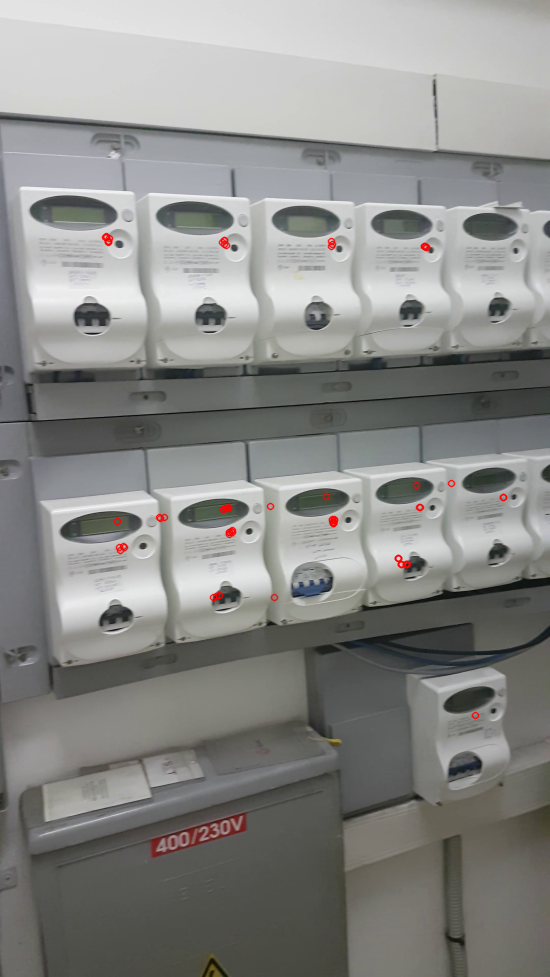
\includegraphics[width=0.15\textwidth]{images/KalmanOrb.png}} \\
    \end{tabular}
    \caption{(a) Kalman filter tracking with Harris corner detector (b) Kalman filter tracking with Blob detector (c) Kalman filter tracking with SIFT detector (d) Kalman filter tracking with ORB detector}
    \label{fig:kalman}
\end{figure}

\section{Conclusion}
\label{sec:conclusion}
This paper proposed a method to identify and track characteristics over several frames, using settings that may be adjusted dynamically through the command line or a configuration file.
The feature recognition and tracking algorithms used are entirely dependent on the scene and the device's processing capabilities. 

To conclude, basic feature detectors may be too naive in noisy or demanding environments such as the one portrayed in the test video.
Although the blob detector is an interesting approach, it is neither agnostic, nor is it rotation or size invariant.
Furthermore, more complicated feature detectors have been demonstrated to be more rigorous, although this comes at a cost.
Therefore if a precise system needs to be developed and a lot of processing power is available, then SIFT is definitely the way to go; however, if resources are limited, then ORB is a good alternative to SIFT, which is a less accurate but still a quite robust feature detector. 
To further improve the overall project, in particular to expand the Kalman filter performances, it would be interesting to integrate it with a sensor capable of providing the object's position.
Finally, it would be delightful to experiment artificial neural networks features to see how they perform in comparison to traditional features and how they could help to improve the algorithm's performance in the future.

\bibliographystyle{IEEEtran}
\bibliography{bibliography/bibliography}

\ifCLASSOPTIONcaptionsoff
  \newpage
\fi

\end{document}